\documentclass[13pt]{beamer}
%
% Choose how your presentation looks.
%
% For more themes, color themes and font themes, see:
% http://deic.uab.es/~iblanes/beamer_gallery/index_by_theme.html
%
\mode<presentation>
{
  \usetheme{CambridgeUS}     % or try Darmstadt, Madrid, Warsaw, ...
  \usecolortheme{beaver} % or try albatross, beaver, crane, ...
  \usefonttheme{default}  % or try serif, structurebold, ...
  \setbeamertemplate{navigation symbols}{}
  \setbeamertemplate{caption}[numbered]
} 

\usepackage[english]{babel}
\usepackage[utf8x]{inputenc}
\usepackage{xcolor}
\usepackage{multicol}
\usepackage{tikz}
\usepackage{tikz-uml}
\tikzumlset{font=\footnotesize\ttfamily, class width=6ex}
\usepackage{hyperref}

\usepackage{listings}
\definecolor{codegreen}{rgb}{0,0.6,0}
\definecolor{codegray}{rgb}{0.5,0.5,0.5}
\definecolor{codepurple}{rgb}{0.58,0,0.82}
\definecolor{backcolour}{rgb}{0.95,0.95,0.92}

\lstdefinestyle{myCustomCppStyle}{
  language=C++,
  numbers=left,
  stepnumber=1,
  numbersep=9pt,
  tabsize=2,
  showspaces=false,
  showstringspaces=false
}

\lstset{basicstyle=\tiny,style=myCustomCppStyle}

\lstdefinestyle{mystyle}{
    backgroundcolor=\color{backcolour},   
    commentstyle=\color{codegreen},
    keywordstyle=\color{magenta},
    numberstyle=\tiny\color{codegray},
    stringstyle=\color{codepurple},
    basicstyle=\ttfamily\footnotesize,
    breakatwhitespace=false,         
    breaklines=true,                 
    captionpos=b,                    
    keepspaces=true,                 
    numbers=left,                    
    numbersep=5pt,                  
    showspaces=false,                
    showstringspaces=false,
    showtabs=false,                  
    tabsize=1
}

\lstset{style=mystyle}

\usepackage{graphicx}
\graphicspath{ {./images/} }

\usepackage{tikz}
\usetikzlibrary{decorations.text}
\usetikzlibrary{shapes.geometric, arrows, positioning, calc, matrix}

\tikzset{
  basic box/.style={
    shape=rectangle, rounded corners, align=center,
    draw=#1, fill=#1!25},
  header node/.style={
    Minimum Width=header nodes,
    font=\strut\Large\ttfamily,
    text depth=+0pt,
    fill=white, draw},
  header/.style={%
    inner ysep=+1.5em,
    append after command={
      \pgfextra{\let\TikZlastnode\tikzlastnode}
      node [header node] (header-\TikZlastnode) at (\TikZlastnode.north) {#1}
      node [span=(\TikZlastnode)(header-\TikZlastnode)] at (fit bounding box) (h-\TikZlastnode) {}
    }
  },
  hv/.style={to path={-|(\tikztotarget)\tikztonodes}},
  vh/.style={to path={|-(\tikztotarget)\tikztonodes}},
  fat blue line/.style={ultra thick, blue}
}

\definecolor{mygray}{RGB}{208,208,208}
\definecolor{mymagenta}{RGB}{226,0,116}
\newcommand*{\mytextstyle}{\sffamily\Large\bfseries\color{black!85}}
\newcommand{\arcarrow}[3]{%
   % inner radius, middle radius, outer radius, start angle,
   % end angle, tip protusion angle, options, text
   \pgfmathsetmacro{\rin}{1.7}
   \pgfmathsetmacro{\rmid}{2.2}
   \pgfmathsetmacro{\rout}{2.7}
   \pgfmathsetmacro{\astart}{#1}
   \pgfmathsetmacro{\aend}{#2}
   \pgfmathsetmacro{\atip}{5}
   \fill[mygray, very thick] (\astart+\atip:\rin)
                         arc (\astart+\atip:\aend:\rin)
      -- (\aend-\atip:\rmid)
      -- (\aend:\rout)   arc (\aend:\astart+\atip:\rout)
      -- (\astart:\rmid) -- cycle;
   \path[
      decoration = {
         text along path,
         text = {|\mytextstyle|#3},
         text align = {align = center},
         raise = -1.0ex
      },
      decorate
   ](\astart+\atip:\rmid) arc (\astart+\atip:\aend+\atip:\rmid);
}
\title[Design Pattern]{Creational Design Pattern}
\author{Hung Tran}
\institute{Fpt software}
\date{\today}

\begin{document}

\begin{frame}
  \titlepage
\end{frame}

% Uncomment these lines for an automatically generated outline.
\begin{frame}{Outline}
  \tableofcontents
\end{frame}

\section{Creational Pattern Overview}

\begin{frame}{Creational Pattern Overview}
	\begin{center}
	\textcolor{blue}{\textbf{Construction process of an object.}}
	\end{center}
	\begin{itemize}
		\setlength\itemsep{1em}
		\item \textbf{Singleton}: Ensure only one instance.
		\item \textbf{Factory Method}: Create instance without depending on its concrete type.
		\item \textbf{Object pool}: Reuse existing instances.
		\item \textbf{Abstract factory}: Create instances from a specific family.
		\item \textbf{Prototype}: Clone existing objects from a prototype.
		\item \textbf{Builder}: Construct a complex object step by step.
	\end{itemize}
\end{frame}

\section{Object Pool Design Pattern}

\begin{frame}{Game Example}
\end{frame}

\begin{frame}{Factory Pattern}
\begin{itemize}
\item Always create new instance
\end{itemize}
\end{frame}

\begin{frame}{The Intent of Object Pool Design Pattern}
	\begin{center}
	\textcolor{blue}{\textbf{Improve performance and memory use by reusing objects from fixed pool instead of allocating and freeing them repetitively.}}
	\end{center}
\end{frame}

\begin{frame}{Structure of Object Pool Design Pattern}
	\begin{center}
	\begin{tikzpicture}
	\umlemptyclass[x=0,y=0]{Clients}
	\umlclass[x=8,y=0]{ObjectPool}{pool: vector}{GetInstance() \\ Acquire() \\ Release()}
	\umlclass[x=8,y=-4]{SharedObject}{}{MethodA() \\ MethodB()}
	\umluniassoc[pos=0.95, align=right, name=uniassoc,]{ObjectPool}{SharedObject}
	\umluniassoc[pos=0.95, align=right, name=uniassoc, arg1=requests]{Clients}{ObjectPool}
	\umluniassoc[geometry = |-,pos=0.95, align=right, name=uniassoc, arg1=uses]{Clients}{SharedObject}
	\end{tikzpicture}	
	\end{center}
\end{frame}

\begin{frame}{How to Implement of Object Pool Design Pattern?}
	\begin{itemize}
		\setlength\itemsep{1em}
		\item \emph{ObjectPool} class maintains an array or a list of \emph{SharedObject} instances
		\item \emph{SharedObject} instances are not created by Clients; instead they use the \emph{ObjectPool} class
		\item Objects are constructed when: The program starts, The pool is empty, An existing object is not available.
		\item For the last case, the pool can be \emph{grow dynamically}.
		\item ObjectPool should have \emph{only one instance} (Singleton or Monostate)
	\end{itemize}
\end{frame}

\begin{frame}{How to Implement of Object Pool Design Pattern?}
	\begin{itemize}
		\setlength\itemsep{1em}
		\item The clients acquire a \emph{SharedObject} instance by invoking a factory method in the pool.
		\item When the clients gets a \emph{SharedObject} instance, it is either removed from the \emph{ObjectPool} or marked as used.
		\item The clients may manually return a \emph{SharedObject} to the \emph{ObjectPool} or t may be done automatically.
		\item The instance can be used again.
	\end{itemize}
\end{frame}

\begin{frame}{How to Implement of Object Pool Design Pattern?}
	\begin{itemize}
		\setlength\itemsep{1em}
		\item The Pool object instance can be reset: before giving it to the client or after it is returned to the pool.
		\item The ObjectPool is responsible for deleting the pooled instances
		\item These instances are usually deleted at the end of the program.
		\item To avoid tight coupling with concreate pooled objects, ObjectPool can use a factory to instantiate them.
	\end{itemize}
\end{frame}

\begin{frame}{Modify existing code problem}
	\begin{center}
	\begin{tikzpicture}
	\umlemptyclass[type=abstract,x=0,y=0]{Product}
	\umlemptyclass[x=0,y=-3]{ConcreteProduct}
	\umlinherit{ConcreteProduct}{Product}
	\umlclass[x=6,y=0]{Creator}{}{AnOperation():Product*}
	\umluniassoc[geometry = -|,pos=0.95, align=right, name=uniassoc]{Creator}{Product}
	\umluniassoc[geometry = -|,pos=0.95, align=right, geometry = -|-, name=uniassoc]{Creator}{ConcreteProduct}
	\end{tikzpicture}	
	\end{center}
	\begin{itemize}
	\item Operation() method returns ConcreteProduct object
	\item Add more ConcreteProduct class, modify AnOperation() method
	\item End up with if else condition.
	\item Always return the same class (using new operator)
	\end{itemize}
\end{frame}

\begin{frame}{Class Diagram Explaining}
\begin{center}
\begin{tikzpicture}
	\umlemptyclass[type=abstract,x=0,y=1]{Product}
	\umlemptyclass[x=-2,y=-2]{ConcreteProduct}
	\umlemptyclass[x=2,y=-2]{ConcreteProduct1}
	\umlinherit[geometry=-|]{ConcreteProduct}{Product}
	\umlinherit[geometry=-|]{ConcreteProduct1}{Product}
	
	\umlclass[type=abstract,x=5,y=1]{Creator}{m\_pProduct: Product*}{\umlvirt{Create()} \\ AnOperation()}
	\umlclass[x=3,y=-4]{ConcreteCreator}{}{Create()}
	\umlclass[x=7,y=-4]{ConcreteCreator1}{}{Create()}
	\umlinherit[geometry=-|]{ConcreteCreator}{Creator}
	\umlinherit[geometry=-|]{ConcreteCreator1}{Creator}
	
	\umluniassoc[geometry=|-, color=green]{Creator}{Product}
	
	\umlimport[geometry = -|, weight = 0.5, color=blue]{ConcreteCreator}{ConcreteProduct}
	\umlimport[geometry = |-, weight = 0.5, color=red]{ConcreteCreator1}{ConcreteProduct1}
\end{tikzpicture}	
\end{center}
\end{frame}

\begin{frame}{Create a ConcreteProduct object}
\begin{columns}[T]
\begin{column}{.4\textwidth}
\lstset{basicstyle=\tiny,style=myCustomCppStyle}
main.cpp
\lstinputlisting{./examples/basicImplementation/factoryBasics/main.cpp}
\end{column}
\begin{column}{.6\textwidth}
	\begin{itemize}
		\setlength\itemsep{1em}
		\item Create() Method (or factory method) is overridden in derived classes.
		\item The dependency on ConcreteProduct is no longer required
		\item AnOperation method calls Create() method.
		\item With the main function, which Create() method will invoke?
		\item No need to modify the AnOperation()
		\item Create() method behaves like virtual constructor
	\end{itemize}
\end{column}
\end{columns}
\end{frame}

\begin{frame}{Real World Example: Application Framework?}
	\textcolor{blue}{We want to create an framework!}	
	\begin{itemize}
		\setlength\itemsep{1em}
		\item The programmer can create an Application based on App framework.
		\item Framework provides managing different kinds of documents.
		\item Framework provides infrastructure of application.
		\item By using app framework, programmer can create an application which can display different kinds of data (\textcolor{red}{Text or Graphics}).
		\item To manage the data, the framework provides support through which is easy to maintain data.
		\item We add \textcolor{red}{Application class} for managing data and display them.
		\item We need add an \textcolor{red}{Document class} that Application manages
	\end{itemize}
\end{frame}

\begin{frame}{Real World Example: Application Framework?}
\begin{itemize}
	\setlength\itemsep{1em}
	\item Application class uses the features of Document class (display them).
	\item However, Application does not know what kind of data is.
	\item Document class need to be abstract in our framework.
	\item \textbf{Document class has methods Read(), Write() which are overridden in derived classes.}
	\item \textbf{Application class uses the features of Document class.}
\end{itemize}
\begin{center}
\begin{tikzpicture}
	\umlclass[type=abstract,x=0,y=0]{Document}{}{\umlvirt{Write()} \\ \umlvirt{Read()}}
	\umlclass[x=5,y=0]{Application}{}{}
	\umluniassoc[geometry=|-]{Application}{Document}
\end{tikzpicture}	
\end{center}
\end{frame}

\begin{frame}{Using Framework for managing data}
\begin{itemize}
	\setlength\itemsep{1em}
	\item Programmer want to use the framework for managing the Text data.
	\item Create a class Text which is derived class of Document class.
	\item Application can use Text through Document class.
\end{itemize}
\begin{center}
\begin{tikzpicture}
	\umlclass[type=abstract,x=0,y=0]{Document}{}{\umlvirt{Write()} \\ \umlvirt{Read()}}
	\umlclass[x=0,y=-2.5]{Text}{}{Write() \\ Read()}
	\umlinherit[geometry=--]{Text}{Document}
	
	\umlclass[x=6,y=0]{Application}{}{New() \\ Open() \\ Save()}
	\umluniassoc[geometry=|-]{Application}{Document}
\end{tikzpicture}	
\end{center}
\end{frame}

\begin{frame}{Adding SpreadSheet class}
\begin{itemize}
	\setlength\itemsep{1em}
	\item New(), Open(), Save() are tight coupled with Text class.
	\item Adding new Document class, change the Application class.
	\item The framework does not allow modifying.
\end{itemize}
\begin{center}
\begin{tikzpicture}
	\umlclass[type=abstract,x=0,y=0]{Document}{}{\umlvirt{Write()} \\ \umlvirt{Read()}}
	\umlclass[x=-2,y=-2.5]{Text}{}{Write() \\ Read()}
	\umlclass[x=2,y=-2.5]{SpreadSheet}{}{Write() \\ Read()}
	\umlinherit[geometry=-|]{Text}{Document}
	\umlinherit[geometry=-|]{SpreadSheet}{Document}
	
	\umlclass[x=6,y=0]{Application}{}{New() \\ Open() \\ Save()}
	\umluniassoc[geometry=|-]{Application}{Document}
\end{tikzpicture}	
\end{center}
\end{frame}

\begin{frame}{App framework with factory method}
\begin{center}
\begin{tikzpicture}
	\umlclass[type=abstract,x=0,y=1]{Document}{}{\umlvirt{Read()} \\ \umlvirt{Write()}}
	\umlemptyclass[x=-2,y=-2]{Text}
	\umlemptyclass[x=2,y=-2]{SpreadSheet}
	\umlinherit[geometry=-|]{Text}{Document}
	\umlinherit[geometry=-|]{SpreadSheet}{Document}
	
	\umlclass[x=5,y=1]{Application}{m\_pDocument: Document*}{\umlvirt{Create()}: Document* \\ New() \\ Open() \\ Save()}
	\umlclass[x=2,y=-4]{TextApp}{}{Create(): Document*}
	\umlclass[x=7.3,y=-4]{SpreadSheetApp}{}{Create(): Document*}
	\umlinherit[geometry=-|]{TextApp}{Application}
	\umlinherit[geometry=-|]{SpreadSheetApp}{Application}
	
	\umluniassoc[geometry=|-, color=green]{Application}{Document}
	
	\umlimport[geometry = -|, weight = 0.5, color=blue]{TextApp}{Text}
	\umlimport[geometry = |-, weight = 0.5, color=red]{SpreadSheetApp}{SpreadSheet}
\end{tikzpicture}	
\end{center}
\end{frame}

\begin{frame}{The Intent of Factory Method Design Pattern}
	\begin{center}
	\textcolor{blue}{\textbf{Define an interface for creating an object, but let subclasses which class to instantitate. Factory method lets class defer instantiation to subclasses.}}
	\end{center}
	\begin{itemize}
	\item Application class is an interface.
	\item Create() method is factory method.
	\item The subclasses (TextApp and SpreadSheetApp) instantiate objects.
	\end{itemize}
\end{frame}

\begin{frame}{Resource Management}
\begin{columns}[T]
\begin{column}{.4\textwidth}
\lstset{basicstyle=\tiny,style=myCustomCppStyle}
\lstinputlisting{./examples/appFramework/appFrame//TextApplication.cpp}
\end{column}
\begin{column}{.6\textwidth}
	\begin{itemize}
		\setlength\itemsep{1em}
		\item \textcolor{red}{How to free the instance?}
		\item Using smart pointers
	\end{itemize}
\end{column}
\end{columns}
\end{frame}

\begin{frame}{Using smart pointer}
\begin{center}
\begin{tikzpicture}
	\umlclass[type=abstract,x=0,y=1]{Document}{}{\umlvirt{Read()} \\ \umlvirt{Write()}}
	\umlemptyclass[x=-2,y=-2]{Text}
	\umlemptyclass[x=2,y=-2]{SpreadSheet}
	\umlinherit[geometry=-|]{Text}{Document}
	\umlinherit[geometry=-|]{SpreadSheet}{Document}
	
	\umlclass[x=5,y=1]{Application}{m\_pDocument: unique\_ptr<Document>}{\umlvirt{Create()}: unique\_ptr<Document> \\ New() \\ Open() \\ Save()}
	\umlclass[x=2,y=-4]{TextApp}{}{Create(): unique}
	\umlclass[x=7.3,y=-4]{SpreadSheetApp}{}{Create(): unique}
	\umlinherit[geometry=-|]{TextApp}{Application}
	\umlinherit[geometry=-|]{SpreadSheetApp}{Application}
	
	\umluniassoc[geometry=|-, color=green]{Application}{Document}
	
	\umlimport[geometry = -|, weight = 0.5, color=blue]{TextApp}{Text}
	\umlimport[geometry = |-, weight = 0.5, color=red]{SpreadSheetApp}{SpreadSheet}
\end{tikzpicture}
\end{center}
\end{frame}

\begin{frame}{Add new Document, add more Application?}
	\textcolor{blue}{How to create multiple instances without creating corresponding application class?}	
	\begin{center}
	\textcolor{red}{\textbf{Using Parameterized Factory}}
	\end{center}
\end{frame}

\begin{frame}{What if you want to read different kinds of document?}
\begin{center}
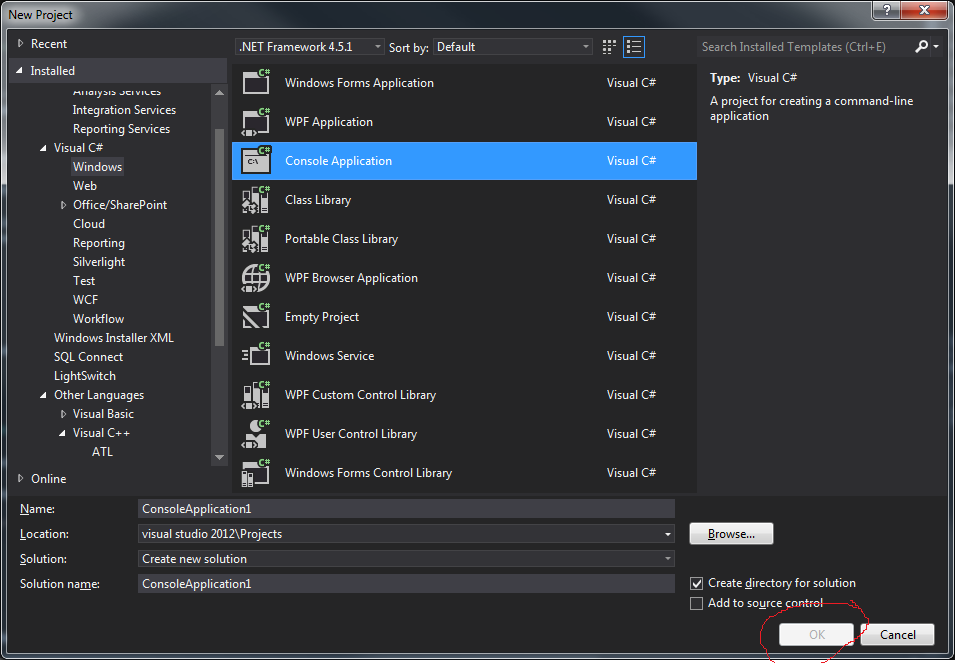
\includegraphics[scale=0.25]{./images/visualDialog.png}
\end{center}

\begin{itemize}
	\setlength\itemsep{1em}
	\item Like dialog shows options which clients can chose.
	\item You need to know how many applications before implementations.
	\item Input Type through user interface.
\end{itemize}
\end{frame}

\begin{frame}{Classes structure: Parameterized Factory}
\begin{center}
\begin{tikzpicture}
	\umlclass[type=abstract,x=-1.5,y=2]{Document}{}{\umlvirt{Read()} \\ \umlvirt{Write()}}
	\umlemptyclass[x=-3,y=-2]{Text}
	\umlemptyclass[x=1,y=-2]{SpreadSheet}
	\umlinherit[geometry=-|]{Text}{Document}
	\umlinherit[geometry=-|]{SpreadSheet}{Document}
	
	\umlclass[x=3,y=0]{DocFactory}{}{Create(Type): Document*}
	\umlclass[x=7,y=-2]{Application}{DocFactory}{New() \\ Open() \\ Save()}
	\umluniassoc[geometry=|-, color=green]{Application}{DocFactory}
	\umlimport[geometry = -|, weight = 0.5, color=blue]{DocFactory}{Text}
	\umlimport[geometry = |-, weight = 0.5, color=red]{DocFactory}{SpreadSheet}
\end{tikzpicture}
\end{center}
\end{frame}

\iffalse
\begin{frame}{App framework: parameterized Factory}
\begin{columns}[T]
\begin{column}{.45\textwidth}
\lstset{basicstyle=\tiny,style=myCustomCppStyle}
Document.h
\lstinputlisting{./examples/parameterizedFactory/paraFact/Document.h}
TextDocument.h
\lstinputlisting{./examples/parameterizedFactory/paraFact/TextDocument.h}
\end{column}

\begin{column}{.45\textwidth}
\lstset{basicstyle=\tiny,style=myCustomCppStyle}
TextDocument.cpp
\lstinputlisting{./examples/parameterizedFactory/paraFact/TextDocument.cpp}
\end{column}
\end{columns}
\end{frame}

\begin{frame}{App framework: parameterized Factory}
\begin{columns}[T]
\begin{column}{.45\textwidth}
\lstset{basicstyle=\tiny,style=myCustomCppStyle}
SpreadSheetDocument.h
\lstinputlisting{./examples/parameterizedFactory/paraFact/SpreadSheetDocument.h}
SpreadSheetDocument.cpp
\lstinputlisting{./examples/parameterizedFactory/paraFact/SpreadSheetDocument.cpp}
\end{column}

\begin{column}{.45\textwidth}
\lstset{basicstyle=\tiny,style=myCustomCppStyle}
\end{column}
\end{columns}
\end{frame}

\begin{frame}{App framework: parameterized Factory}
\begin{columns}[T]
\begin{column}{.45\textwidth}
\lstset{basicstyle=\tiny,style=myCustomCppStyle}
Application.h
\lstinputlisting{./examples/parameterizedFactory/paraFact/Application.h}
\end{column}

\begin{column}{.45\textwidth}
\lstset{basicstyle=\tiny,style=myCustomCppStyle}
Application.cpp
\lstinputlisting{./examples/parameterizedFactory/paraFact/Application.cpp}
\end{column}
\end{columns}
\end{frame}
\fi

\begin{frame}{Pros and Cons}
\begin{columns}[T]
\begin{column}{.45\textwidth}
	\begin{center}
	\textcolor{blue}{\textbf{Pros}}
	\end{center}
	\begin{itemize}
		\item Instances can be created at runtime
		\item Promote loose coupling
		\item Construction becomes simple due to abstraction
		\item Construction becomes encapsulated
		\item May not return new instance every time (return a cache instance), useful for object pool
	\end{itemize}
\end{column}
\begin{column}{.45\textwidth}
	\begin{center}
	\textcolor{blue}{\textbf{Cons}}
	\end{center}
		\begin{itemize}
		\setlength\itemsep{1em}
		\item Every new product class may require a corresponding factory class.
	\end{itemize}
\end{column}
\end{columns}
\end{frame}

\begin{frame}{Where to use?}	
	\begin{itemize}
		\setlength\itemsep{1em}
		\item A class does not know which instance it needs at runtime.
		\item A class does not want to depend on concrete classes that it uses.
		\item You want to encapsulate the creation process.
	\end{itemize}
\end{frame}

\end{document}
